\chapter{Chapter XXXI}

\begin{verse}
Once more unto the breach, dear friends, once more,\\
Or, close the wall up with our English dead.\\
-------And you, good yeomen,\\
Whose limbs were made in England, show us here\\
The mettle of your pasture--let us swear\\
That you are worth your breeding.\\!
\attrib{King Henry V}
\end{verse}

\lettrine{C}{edric}, although not greatly confident in Ulrica's message,
omitted not
to communicate her promise to the Black Knight and Locksley. They were
well pleased to find they had a friend within the place, who might, in
the moment of need, be able to facilitate their entrance, and readily
agreed with the Saxon that a storm, under whatever disadvantages, ought
to be attempted, as the only means of liberating the prisoners now in
the hands of the cruel Front-de-Boeuf.

``The royal blood of Alfred is endangered,'' said Cedric.

``The honour of a noble lady is in peril,'' said the Black Knight.

``And, by the Saint Christopher at my baldric,'' said the good yeoman,
``were there no other cause than the safety of that poor faithful knave,
Wamba, I would jeopard a joint ere a hair of his head were hurt.''

``And so would I,'' said the Friar; ``what, sirs! I trust well that a
fool--I mean, d'ye see me, sirs, a fool that is free of his guild and
master of his craft, and can give as much relish and flavour to a cup of
wine as ever a flitch of bacon can--I say, brethren, such a fool shall
never want a wise clerk to pray for or fight for him at a strait, while
I can say a mass or flourish a partisan.'' And with that he made his
heavy halberd to play around his head as a shepherd boy flourishes his
light crook.

``True, Holy Clerk,'' said the Black Knight, ``true as if Saint Dunstan
himself had said it.--And now, good Locksley, were it not well that
noble Cedric should assume the direction of this assault?''

``Not a jot I,'' returned Cedric; ``I have never been wont to study
either how to take or how to hold out those abodes of tyrannic power,
which the Normans have erected in this groaning land. I will fight among
the foremost; but my honest neighbours well know I am not a trained
soldier in the discipline of wars, or the attack of strongholds.''

``Since it stands thus with noble Cedric,'' said Locksley, ``I am most
willing to take on me the direction of the archery; and ye shall hang me
up on my own Trysting-tree, an the defenders be permitted to show
themselves over the walls without being stuck with as many shafts as
there are cloves in a gammon of bacon at Christmas.''

``Well said, stout yeoman,'' answered the Black Knight; ``and if I be
thought worthy to have a charge in these matters, and can find among
these brave men as many as are willing to follow a true English knight,
for so I may surely call myself, I am ready, with such skill as my
experience has taught me, to lead them to the attack of these walls.''

The parts being thus distributed to the leaders, they commenced the
first assault, of which the reader has already heard the issue.

When the barbican was carried, the Sable Knight sent notice of the happy
event to Locksley, requesting him at the same time, to keep such a
strict observation on the castle as might prevent the defenders from
combining their force for a sudden sally, and recovering the outwork
which they had lost. This the knight was chiefly desirous of avoiding,
conscious that the men whom he led, being hasty and untrained
volunteers, imperfectly armed and unaccustomed to discipline, must, upon
any sudden attack, fight at great disadvantage with the veteran soldiers
of the Norman knights, who were well provided with arms both defensive
and offensive; and who, to match the zeal and high spirit of the
besiegers, had all the confidence which arises from perfect discipline
and the habitual use of weapons.

The knight employed the interval in causing to be constructed a sort of
floating bridge, or long raft, by means of which he hoped to cross the
moat in despite of the resistance of the enemy. This was a work of some
time, which the leaders the less regretted, as it gave Ulrica leisure to
execute her plan of diversion in their favour, whatever that might be.

When the raft was completed, the Black Knight addressed the
besiegers:--``It avails not waiting here longer, my friends; the sun is
descending to the west--and I have that upon my hands which will not
permit me to tarry with you another day. Besides, it will be a marvel if
the horsemen come not upon us from York, unless we speedily accomplish
our purpose. Wherefore, one of ye go to Locksley, and bid him commence a
discharge of arrows on the opposite side of the castle, and move forward
as if about to assault it; and you, true English hearts, stand by me,
and be ready to thrust the raft endlong over the moat whenever the
postern on our side is thrown open. Follow me boldly across, and aid me
to burst yon sallyport in the main wall of the castle. As many of you as
like not this service, or are but ill armed to meet it, do you man the
top of the outwork, draw your bow-strings to your ears, and mind you
quell with your shot whatever shall appear to man the rampart--Noble
Cedric, wilt thou take the direction of those which remain?''

``Not so, by the soul of Hereward!'' said the Saxon; ``lead I cannot;
but may posterity curse me in my grave, if I follow not with the
foremost wherever thou shalt point the way--The quarrel is mine, and
well it becomes me to be in the van of the battle.''

``Yet, bethink thee, noble Saxon,'' said the knight, ``thou hast neither
hauberk, nor corslet, nor aught but that light helmet, target, and
sword.''

``The better!'' answered Cedric; ``I shall be the lighter to climb these
walls. And,--forgive the boast, Sir Knight,--thou shalt this day see the
naked breast of a Saxon as boldly presented to the battle as ever ye
beheld the steel corslet of a Norman.''

``In the name of God, then,'' said the knight, ``fling open the door,
and launch the floating bridge.''

The portal, which led from the inner-wall of the barbican to the moat,
and which corresponded with a sallyport in the main wall of the castle,
was now suddenly opened; the temporary bridge was then thrust forward,
and soon flashed in the waters, extending its length between the castle
and outwork, and forming a slippery and precarious passage for two men
abreast to cross the moat. Well aware of the importance of taking the
foe by surprise, the Black Knight, closely followed by Cedric, threw
himself upon the bridge, and reached the opposite side. Here he began to
thunder with his axe upon the gate of the castle, protected in part from
the shot and stones cast by the defenders by the ruins of the former
drawbridge, which the Templar had demolished in his retreat from the
barbican, leaving the counterpoise still attached to the upper part of
the portal. The followers of the knight had no such shelter; two were
instantly shot with cross-bow bolts, and two more fell into the moat;
the others retreated back into the barbican.

The situation of Cedric and of the Black Knight was now truly dangerous,
and would have been still more so, but for the constancy of the archers
in the barbican, who ceased not to shower their arrows upon the
battlements, distracting the attention of those by whom they were
manned, and thus affording a respite to their two chiefs from the storm
of missiles which must otherwise have overwhelmed them. But their
situation was eminently perilous, and was becoming more so with every
moment.

``Shame on ye all!'' cried De Bracy to the soldiers around him; ``do ye
call yourselves cross-bowmen, and let these two dogs keep their station
under the walls of the castle?--Heave over the coping stones from the
battlements, an better may not be--Get pick-axe and levers, and down
with that huge pinnacle!'' pointing to a heavy piece of stone
carved-work that projected from the parapet.

At this moment the besiegers caught sight of the red flag upon the angle
of the tower which Ulrica had described to Cedric. The stout yeoman
Locksley was the first who was aware of it, as he was hasting to the
outwork, impatient to see the progress of the assault.

``Saint George!'' he cried, ``Merry Saint George for England!--To the
charge, bold yeomen!--why leave ye the good knight and noble Cedric to
storm the pass alone?--make in, mad priest, show thou canst fight for
thy rosary,--make in, brave yeomen!--the castle is ours, we have friends
within--See yonder flag, it is the appointed signal--Torquilstone is
ours!--Think of honour, think of spoil--One effort, and the place is
ours!''

With that he bent his good bow, and sent a shaft right through the
breast of one of the men-at-arms, who, under De Bracy's direction, was
loosening a fragment from one of the battlements to precipitate on the
heads of Cedric and the Black Knight. A second soldier caught from the
hands of the dying man the iron crow, with which he heaved at and had
loosened the stone pinnacle, when, receiving an arrow through his
head-piece, he dropped from the battlements into the moat a dead man.
The men-at-arms were daunted, for no armour seemed proof against the
shot of this tremendous archer.

``Do you give ground, base knaves!'' said De Bracy; ``\,`Mount joye
Saint Dennis!'--Give me the lever!''

And, snatching it up, he again assailed the loosened pinnacle, which was
of weight enough, if thrown down, not only to have destroyed the remnant
of the drawbridge, which sheltered the two foremost assailants, but also
to have sunk the rude float of planks over which they had crossed. All
saw the danger, and the boldest, even the stout Friar himself, avoided
setting foot on the raft. Thrice did Locksley bend his shaft against De
Bracy, and thrice did his arrow bound back from the knight's armour of
proof.

``Curse on thy Spanish steel-coat!'' said Locksley, ``had English smith
forged it, these arrows had gone through, an as if it had been silk or
sendal.'' He then began to call out, ``Comrades! friends! noble Cedric!
bear back, and let the ruin fall.''

His warning voice was unheard, for the din which the knight himself
occasioned by his strokes upon the postern would have drowned twenty
war-trumpets. The faithful Gurth indeed sprung forward on the planked
bridge, to warn Cedric of his impending fate, or to share it with him.
But his warning would have come too late; the massive pinnacle already
tottered, and De Bracy, who still heaved at his task, would have
accomplished it, had not the voice of the Templar sounded close in his
ears:--

``All is lost, De Bracy, the castle burns.''

``Thou art mad to say so!'' replied the knight.

``It is all in a light flame on the western side. I have striven in vain
to extinguish it.''

With the stern coolness which formed the basis of his character, Brian
de Bois-Guilbert communicated this hideous intelligence, which was not
so calmly received by his astonished comrade.

``Saints of Paradise!'' said De Bracy; ``what is to be done? I vow to
Saint Nicholas of Limoges a candlestick of pure gold--''

``Spare thy vow,'' said the Templar, ``and mark me. Lead thy men down,
as if to a sally; throw the postern-gate open--There are but two men who
occupy the float, fling them into the moat, and push across for the
barbican. I will charge from the main gate, and attack the barbican on
the outside; and if we can regain that post, be assured we shall defend
ourselves until we are relieved, or at least till they grant us fair
quarter.''

``It is well thought upon,'' said De Bracy; ``I will play my
part--Templar, thou wilt not fail me?''

``Hand and glove, I will not!'' said Bois-Guilbert. ``But haste thee, in
the name of God!''

De Bracy hastily drew his men together, and rushed down to the
postern-gate, which he caused instantly to be thrown open. But scarce
was this done ere the portentous strength of the Black Knight forced his
way inward in despite of De Bracy and his followers. Two of the foremost
instantly fell, and the rest gave way notwithstanding all their leader's
efforts to stop them.

``Dogs!'' said De Bracy, ``will ye let TWO men win our only pass for
safety?''

``He is the devil!'' said a veteran man-at-arms, bearing back from the
blows of their sable antagonist.

``And if he be the devil,'' replied De Bracy, ``would you fly from him
into the mouth of hell?--the castle burns behind us, villains!--let
despair give you courage, or let me forward! I will cope with this
champion myself.''

And well and chivalrous did De Bracy that day maintain the fame he had
acquired in the civil wars of that dreadful period. The vaulted passage
to which the postern gave entrance, and in which these two redoubted
champions were now fighting hand to hand, rung with the furious blows
which they dealt each other, De Bracy with his sword, the Black Knight
with his ponderous axe. At length the Norman received a blow, which,
though its force was partly parried by his shield, for otherwise never
more would De Bracy have again moved limb, descended yet with such
violence on his crest, that he measured his length on the paved floor.

``Yield thee, De Bracy,'' said the Black Champion, stooping over him,
and holding against the bars of his helmet the fatal poniard with which
the knights dispatched their enemies, (and which was called the dagger
of mercy,)--``yield thee, Maurice de Bracy, rescue or no rescue, or thou
art but a dead man.''

``I will not yield,'' replied De Bracy faintly, ``to an unknown
conqueror. Tell me thy name, or work thy pleasure on me--it shall never
be said that Maurice de Bracy was prisoner to a nameless churl.''

The Black Knight whispered something into the ear of the vanquished.

``I yield me to be true prisoner, rescue or no rescue,'' answered the
Norman, exchanging his tone of stern and determined obstinacy for one of
deep though sullen submission.

``Go to the barbican,'' said the victor, in a tone of authority, ``and
there wait my further orders.''

``Yet first, let me say,'' said De Bracy, ``what it imports thee to
know. Wilfred of Ivanhoe is wounded and a prisoner, and will perish in
the burning castle without present help.''

``Wilfred of Ivanhoe!'' exclaimed the Black Knight--``prisoner, and
perish!--The life of every man in the castle shall answer it if a hair
of his head be singed--Show me his chamber!''

``Ascend yonder winding stair,'' said De Bracy; ``it leads to his
apartment--Wilt thou not accept my guidance?'' he added, in a submissive
voice.

``No.~To the barbican, and there wait my orders. I trust thee not, De
Bracy.''

During this combat and the brief conversation which ensued, Cedric, at
the head of a body of men, among whom the Friar was conspicuous, had
pushed across the bridge as soon as they saw the postern open, and drove
back the dispirited and despairing followers of De Bracy, of whom some
asked quarter, some offered vain resistance, and the greater part fled
towards the court-yard. De Bracy himself arose from the ground, and cast
a sorrowful glance after his conqueror. ``He trusts me not!'' he
repeated; ``but have I deserved his trust?'' He then lifted his sword
from the floor, took off his helmet in token of submission, and, going
to the barbican, gave up his sword to Locksley, whom he met by the way.

As the fire augmented, symptoms of it became soon apparent in the
chamber, where Ivanhoe was watched and tended by the Jewess Rebecca. He
had been awakened from his brief slumber by the noise of the battle; and
his attendant, who had, at his anxious desire, again placed herself at
the window to watch and report to him the fate of the attack, was for
some time prevented from observing either, by the increase of the
smouldering and stifling vapour. At length the volumes of smoke which
rolled into the apartment--the cries for water, which were heard even
above the din of the battle made them sensible of the progress of this
new danger.

``The castle burns,'' said Rebecca; ``it burns!--What can we do to save
ourselves?''

``Fly, Rebecca, and save thine own life,'' said Ivanhoe, ``for no human
aid can avail me.''

``I will not fly,'' answered Rebecca; ``we will be saved or perish
together--And yet, great God!--my father, my father--what will be his
fate!''

At this moment the door of the apartment flew open, and the Templar
presented himself,--a ghastly figure, for his gilded armour was broken
and bloody, and the plume was partly shorn away, partly burnt from his
casque. ``I have found thee,'' said he to Rebecca; ``thou shalt prove I
will keep my word to share weal and woe with thee--There is but one path
to safety, I have cut my way through fifty dangers to point it to
thee--up, and instantly follow me!''\footnote{The author has some idea
that this passage is imitated
from the appearance of Philidaspes, before the divine Mandane, when the
city of Babylon is on fire, and he proposes to carry her from the
flames. But the theft, if there be one, would be rather too severely
punished by the penance of searching for the original passage through
the interminable volumes of the Grand Cyrus.}

``Alone,'' answered Rebecca, ``I will not follow thee. If thou wert born
of woman--if thou hast but a touch of human charity in thee--if thy
heart be not hard as thy breastplate--save my aged father--save this
wounded knight!''

``A knight,'' answered the Templar, with his characteristic calmness,
``a knight, Rebecca, must encounter his fate, whether it meet him in the
shape of sword or flame--and who recks how or where a Jew meets with
his?''

``Savage warrior,'' said Rebecca, ``rather will I perish in the flames
than accept safety from thee!''

``Thou shalt not choose, Rebecca--once didst thou foil me, but never
mortal did so twice.''

So saying, he seized on the terrified maiden, who filled the air with
her shrieks, and bore her out of the room in his arms in spite of her
cries, and without regarding the menaces and defiance which Ivanhoe
thundered against him. ``Hound of the Temple--stain to thine Order--set
free the damsel! Traitor of Bois-Guilbert, it is Ivanhoe commands
thee!--Villain, I will have thy heart's blood!''

\begin{figure}
    \centering
    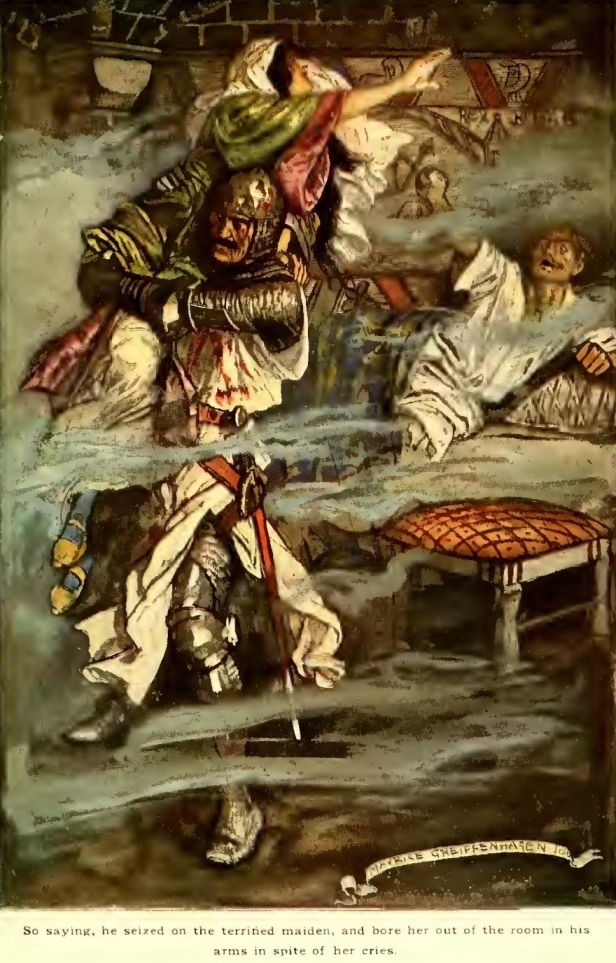
\includegraphics[height=.9\textheight]{ivanhoe/0403m}
    \caption{So saying, he seized on the terrified maiden, and bore her
    out of the room in his arms in spite of her cries.}
\end{figure}

``I had not found thee, Wilfred,'' said the Black Knight, who at that
instant entered the apartment, ``but for thy shouts.''

``If thou be'st true knight,'' said Wilfred, ``think not of me--pursue
yon ravisher--save the Lady Rowena--look to the noble Cedric!''

``In their turn,'' answered he of the Fetterlock, ``but thine is
first.''

And seizing upon Ivanhoe, he bore him off with as much ease as the
Templar had carried off Rebecca, rushed with him to the postern, and
having there delivered his burden to the care of two yeomen, he again
entered the castle to assist in the rescue of the other prisoners.

One turret was now in bright flames, which flashed out furiously from
window and shot-hole. But in other parts, the great thickness of the
walls and the vaulted roofs of the apartments, resisted the progress of
the flames, and there the rage of man still triumphed, as the scarce
more dreadful element held mastery elsewhere; for the besiegers pursued
the defenders of the castle from chamber to chamber, and satiated in
their blood the vengeance which had long animated them against the
soldiers of the tyrant Front-de-Boeuf. Most of the garrison resisted to
the uttermost--few of them asked quarter--none received it. The air was
filled with groans and clashing of arms--the floors were slippery with
the blood of despairing and expiring wretches.

Through this scene of confusion, Cedric rushed in quest of Rowena, while
the faithful Gurth, following him closely through the ``melee'',
neglected his own safety while he strove to avert the blows that were
aimed at his master. The noble Saxon was so fortunate as to reach his
ward's apartment just as she had abandoned all hope of safety, and, with
a crucifix clasped in agony to her bosom, sat in expectation of instant
death. He committed her to the charge of Gurth, to be conducted in
safety to the barbican, the road to which was now cleared of the enemy,
and not yet interrupted by the flames. This accomplished, the loyal
Cedric hastened in quest of his friend Athelstane, determined, at every
risk to himself, to save that last scion of Saxon royalty. But ere
Cedric penetrated as far as the old hall in which he had himself been a
prisoner, the inventive genius of Wamba had procured liberation for
himself and his companion in adversity.

When the noise of the conflict announced that it was at the hottest, the
Jester began to shout, with the utmost power of his lungs, ``Saint
George and the dragon!--Bonny Saint George for merry England!--The
castle is won!'' And these sounds he rendered yet more fearful, by
banging against each other two or three pieces of rusty armour which lay
scattered around the hall.

A guard, which had been stationed in the outer, or anteroom, and whose
spirits were already in a state of alarm, took fright at Wamba's
clamour, and, leaving the door open behind them, ran to tell the Templar
that foemen had entered the old hall. Meantime the prisoners found no
difficulty in making their escape into the anteroom, and from thence
into the court of the castle, which was now the last scene of contest.
Here sat the fierce Templar, mounted on horseback, surrounded by several
of the garrison both on horse and foot, who had united their strength to
that of this renowned leader, in order to secure the last chance of
safety and retreat which remained to them. The drawbridge had been
lowered by his orders, but the passage was beset; for the archers, who
had hitherto only annoyed the castle on that side by their missiles, no
sooner saw the flames breaking out, and the bridge lowered, than they
thronged to the entrance, as well to prevent the escape of the garrison,
as to secure their own share of booty ere the castle should be burnt
down. On the other hand, a party of the besiegers who had entered by the
postern were now issuing out into the court-yard, and attacking with
fury the remnant of the defenders who were thus assaulted on both sides
at once.

Animated, however, by despair, and supported by the example of their
indomitable leader, the remaining soldiers of the castle fought with the
utmost valour; and, being well-armed, succeeded more than once in
driving back the assailants, though much inferior in numbers. Rebecca,
placed on horseback before one of the Templar's Saracen slaves, was in
the midst of the little party; and Bois-Guilbert, notwithstanding the
confusion of the bloody fray, showed every attention to her safety.
Repeatedly he was by her side, and, neglecting his own defence, held
before her the fence of his triangular steel-plated shield; and anon
starting from his position by her, he cried his war-cry, dashed forward,
struck to earth the most forward of the assailants, and was on the same
instant once more at her bridle rein.

Athelstane, who, as the reader knows, was slothful, but not cowardly,
beheld the female form whom the Templar protected thus sedulously, and
doubted not that it was Rowena whom the knight was carrying off, in
despite of all resistance which could be offered.

``By the soul of Saint Edward,'' he said, ``I will rescue her from
yonder over-proud knight, and he shall die by my hand!''

``Think what you do!'' cried Wamba; ``hasty hand catches frog for
fish--by my bauble, yonder is none of my Lady Rowena--see but her long
dark locks!--Nay, an ye will not know black from white, ye may be
leader, but I will be no follower--no bones of mine shall be broken
unless I know for whom.--And you without armour too!--Bethink you, silk
bonnet never kept out steel blade.--Nay, then, if wilful will to water,
wilful must drench.--`Deus vobiscum', most doughty Athelstane!''--he
concluded, loosening the hold which he had hitherto kept upon the
Saxon's tunic.

To snatch a mace from the pavement, on which it lay beside one whose
dying grasp had just relinquished it--to rush on the Templar's band, and
to strike in quick succession to the right and left, levelling a warrior
at each blow, was, for Athelstane's great strength, now animated with
unusual fury, but the work of a single moment; he was soon within two
yards of Bois-Guilbert, whom he defied in his loudest tone.

``Turn, false-hearted Templar! let go her whom thou art unworthy to
touch--turn, limb of a hand of murdering and hypocritical robbers!''

``Dog!'' said the Templar, grinding his teeth, ``I will teach thee to
blaspheme the holy Order of the Temple of Zion;'' and with these words,
half-wheeling his steed, he made a demi-courbette towards the Saxon, and
rising in the stirrups, so as to take full advantage of the descent of
the horse, he discharged a fearful blow upon the head of Athelstane.

Well said Wamba, that silken bonnet keeps out no steel blade. So
trenchant was the Templar's weapon, that it shore asunder, as it had
been a willow twig, the tough and plaited handle of the mace, which the
ill-fated Saxon reared to parry the blow, and, descending on his head,
levelled him with the earth.

``\,`Ha! Beau-seant!'\,'' exclaimed Bois-Guilbert, ``thus be it to the
maligners of the Temple-knights!'' Taking advantage of the dismay which
was spread by the fall of Athelstane, and calling aloud, ``Those who
would save themselves, follow me!'' he pushed across the drawbridge,
dispersing the archers who would have intercepted them. He was followed
by his Saracens, and some five or six men-at-arms, who had mounted their
horses. The Templar's retreat was rendered perilous by the numbers of
arrows shot off at him and his party; but this did not prevent him from
galloping round to the barbican, of which, according to his previous
plan, he supposed it possible De Bracy might have been in possession.

``De Bracy! De Bracy!'' he shouted, ``art thou there?''

``I am here,'' replied De Bracy, ``but I am a prisoner.''

``Can I rescue thee?'' cried Bois-Guilbert.

``No,'' replied De Bracy; ``I have rendered me, rescue or no rescue. I
will be true prisoner. Save thyself--there are hawks abroad--put the
seas betwixt you and England--I dare not say more.''

``Well,'' answered the Templar, ``an thou wilt tarry there, remember I
have redeemed word and glove. Be the hawks where they will, methinks the
walls of the Preceptory of Templestowe will be cover sufficient, and
thither will I, like heron to her haunt.''

Having thus spoken, he galloped off with his followers.

Those of the castle who had not gotten to horse, still continued to
fight desperately with the besiegers, after the departure of the
Templar, but rather in despair of quarter than that they entertained any
hope of escape. The fire was spreading rapidly through all parts of the
castle, when Ulrica, who had first kindled it, appeared on a turret, in
the guise of one of the ancient furies, yelling forth a war-song, such
as was of yore raised on the field of battle by the scalds of the yet
heathen Saxons. Her long dishevelled grey hair flew back from her
uncovered head; the inebriating delight of gratified vengeance contended
in her eyes with the fire of insanity; and she brandished the distaff
which she held in her hand, as if she had been one of the Fatal Sisters,
who spin and abridge the thread of human life. Tradition has preserved
some wild strophes of the barbarous hymn which she chanted wildly amid
that scene of fire and of slaughter:--

\begin{verse}
\flagverse{1.}
Whet the bright steel,\\
Sons of the White Dragon!\\
Kindle the torch,\\
Daughter of Hengist!\\
The steel glimmers not for the carving of the banquet,\\
It is hard, broad, and sharply pointed;\\
The torch goeth not to the bridal chamber,\\
It steams and glitters blue with sulphur.\\
Whet the steel, the raven croaks!\\
Light the torch, Zernebock is yelling!\\
Whet the steel, sons of the Dragon!\\
Kindle the torch, daughter of Hengist! \\!
\flagverse{2.}
The black cloud is low over the thane's castle\\
The eagle screams--he rides on its bosom.\\
Scream not, grey rider of the sable cloud,\\
Thy banquet is prepared!\\
The maidens of Valhalla look forth,\\
The race of Hengist will send them guests.\\
Shake your black tresses, maidens of Valhalla!\\
And strike your loud timbrels for joy!\\
Many a haughty step bends to your halls,\\
Many a helmed head.\\!
\flagverse{3.}
Dark sits the evening upon the thanes castle,\\
The black clouds gather round;\\
Soon shall they be red as the blood of the valiant!\\
The destroyer of forests shall shake his red crest against
them.\\
He, the bright consumer of palaces,\\
Broad waves he his blazing banner,\\
Red, wide and dusky,\\
Over the strife of the valiant:\\
His joy is in the clashing swords and broken bucklers;\\
He loves to lick the hissing blood as it bursts warm from the
wound!\\!
\flagverse{4.}
All must perish!\\
The sword cleaveth the helmet;\\
The strong armour is pierced by the lance;\\
Fire devoureth the dwelling of princes,\\
Engines break down the fences of the battle.\\
All must perish!\\
The race of Hengist is gone--\\
The name of Horsa is no more!\\
Shrink not then from your doom, sons of the sword!\\
Let your blades drink blood like wine;\\
Feast ye in the banquet of slaughter,\\
By the light of the blazing halls!\\
Strong be your swords while your blood is warm,\\
And spare neither for pity nor fear,\\
For vengeance hath but an hour;\\
Strong hate itself shall expire\\
I also must perish!\footnote{Note G. Ulrica's Death Song. See
page~\pageref{noteCXXXI}.}\\!
\end{verse}

The towering flames had now surmounted every obstruction, and rose to
the evening skies one huge and burning beacon, seen far and wide through
the adjacent country. Tower after tower crashed down, with blazing roof
and rafter; and the combatants were driven from the court-yard. The
vanquished, of whom very few remained, scattered and escaped into the
neighbouring wood. The victors, assembling in large bands, gazed with
wonder, not unmixed with fear, upon the flames, in which their own ranks
and arms glanced dusky red. The maniac figure of the Saxon Ulrica was
for a long time visible on the lofty stand she had chosen, tossing her
arms abroad with wild exultation, as if she reined empress of the
conflagration which she had raised. At length, with a terrific crash,
the whole turret gave way, and she perished in the flames which had
consumed her tyrant. An awful pause of horror silenced each murmur of
the armed spectators, who, for the space of several minutes, stirred not
a finger, save to sign the cross. The voice of Locksley was then heard,
``Shout, yeomen!--the den of tyrants is no more! Let each bring his
spoil to our chosen place of rendezvous at the Trysting-tree in the
Harthill-walk; for there at break of day will we make just partition
among our own bands, together with our worthy allies in this great deed
of vengeance.''
